\documentclass[10pt,mathserif]{beamer}

\usepackage{graphicx,amsmath,amssymb,tikz,psfrag}
\usepackage{natbib}

% ------------------------------------------------------------------------
% Packages
% ------------------------------------------------------------------------
\usepackage{amsmath}
\usepackage{tabularx}

% ------------------------------------------------------------------------
% Macros
% ------------------------------------------------------------------------
%~~~~~~~~~~~~~~~
% List shorthand
%~~~~~~~~~~~~~~~
\newcommand{\BIT}{\begin{itemize}}
\newcommand{\EIT}{\end{itemize}}
\newcommand{\BNUM}{\begin{enumerate}}
\newcommand{\ENUM}{\end{enumerate}}
%~~~~~~~~~~~~~~~
% Text with quads around it
%~~~~~~~~~~~~~~~
\newcommand{\qtext}[1]{\quad\text{#1}\quad}
%~~~~~~~~~~~~~~~
% Shorthand for math formatting
%~~~~~~~~~~~~~~~
\newcommand\mbb[1]{\mathbb{#1}}
\newcommand\mbf[1]{\mathbf{#1}}
\def\mc#1{\mathcal{#1}}
\def\mrm#1{\mathrm{#1}}
%~~~~~~~~~~~~~~~
% Common sets
%~~~~~~~~~~~~~~~
\def\reals{\mathbb{R}} % Real number symbol
\def\integers{\mathbb{Z}} % Integer symbol
\def\rationals{\mathbb{Q}} % Rational numbers
\def\naturals{\mathbb{N}} % Natural numbers
\def\complex{\mathbb{C}} % Complex numbers
\def\simplex{\mathcal{S}} % Simplex
%~~~~~~~~~~~~~~~
% Common functions
%~~~~~~~~~~~~~~~
\renewcommand{\exp}[1]{\operatorname{exp}\left(#1\right)} % Exponential
\def\indic#1{\mbb{I}\left({#1}\right)} % Indicator function
\providecommand{\maximize}{\mathop\mathrm{maximize}} % Defining math symbols
\providecommand{\minimize}{\mathop\mathrm{minimize}}
\providecommand{\argmax}{\mathop\mathrm{arg max}}
\providecommand{\argmin}{\mathop\mathrm{arg min}}
\providecommand{\arccos}{\mathop\mathrm{arccos}}
\providecommand{\asinh}{\mathop\mathrm{asinh}}
\providecommand{\dom}{\mathop\mathrm{dom}} % Domain
\providecommand{\range}{\mathop\mathrm{range}} % Range
\providecommand{\diag}{\mathop\mathrm{diag}}
\providecommand{\tr}{\mathop\mathrm{tr}}
\providecommand{\abs}{\mathop\mathrm{abs}}
\providecommand{\card}{\mathop\mathrm{card}}
\providecommand{\sign}{\mathop\mathrm{sign}}
\def\rank#1{\mathrm{rank}({#1})}
\def\supp#1{\mathrm{supp}({#1})}
%~~~~~~~~~~~~~~~
% Common probability symbols
%~~~~~~~~~~~~~~~
\def\E{\mathbb{E}} % Expectation symbol
\def\Earg#1{\E\left[{#1}\right]}
\def\Esubarg#1#2{\E_{#1}\left[{#2}\right]}
\def\P{\mathbb{P}} % Probability symbol
\def\Parg#1{\P\left({#1}\right)}
\def\Psubarg#1#2{\P_{#1}\left[{#2}\right]}
\def\Cov{\mrm{Cov}} % Covariance symbol
\def\Corr{\mrm{Corr}} % Covariance symbol
\def\Covarg#1{\Cov\left[{#1}\right]}
\def\Covsubarg#1#2{\Cov_{#1}\left[{#2}\right]}
\def\Corrsubarg#1#2{\Corr_{#1}\left[{#2}\right]}
\def\Var{\mrm{Var}}
\def\Vararg#1{\Var\left(#1\right)}
\def\Varsubarg#1#2{\Var_{#1}\left(#2\right)}
\newcommand{\family}{\mathcal{P}} % probability family
\newcommand{\eps}{\epsilon}
\def\absarg#1{\left|#1\right|}
\def\msarg#1{\left(#1\right)^{2}}
\def\logarg#1{\log\left(#1\right)}
%~~~~~~~~~~~~~~~
% Distributions
%~~~~~~~~~~~~~~~
\def\Gsn{\mathcal{N}}
\def\Ber{\textnormal{Ber}}
\def\Bin{\textnormal{Bin}}
\def\Unif{\textnormal{Unif}}
\def\Mult{\textnormal{Mult}}
\def\Cat{\textnormal{Cat}}
\def\Gam{\textnormal{Gam}}
\def\InvGam{\textnormal{InvGam}}
\def\NegMult{\textnormal{NegMult}}
\def\Dir{\textnormal{Dir}}
\def\Lap{\textnormal{Laplace}}
\def\Bet{\textnormal{Beta}}
\def\Poi{\textnormal{Poi}}
\def\HypGeo{\textnormal{HypGeo}}
\def\GEM{\textnormal{GEM}}
\def\BP{\textnormal{BP}}
\def\DP{\textnormal{DP}}
\def\BeP{\textnormal{BeP}}
%~~~~~~~~~~~~~~~
% Theorem-like environments
%~~~~~~~~~~~~~~~

%-----------------------
% Probability sets
%-----------------------
\newcommand{\X}{\mathcal{X}}
\newcommand{\Y}{\mathcal{Y}}
\newcommand{\D}{\mathcal{D}}
\newcommand{\Scal}{\mathcal{S}}
%-----------------------
% vector notation
%-----------------------
\newcommand{\bx}{\mathbf{x}}
\newcommand{\by}{\mathbf{y}}
\newcommand{\bt}{\mathbf{t}}
\newcommand{\xbar}{\overline{x}}
\newcommand{\Xbar}{\overline{X}}
\newcommand{\tolaw}{\xrightarrow{\mathcal{L}}}
\newcommand{\toprob}{\xrightarrow{\mathbb{P}}}
\newcommand{\laweq}{\overset{\mathcal{L}}{=}}
\newcommand{\F}{\mathcal{F}}


\mode<presentation>
{
\usetheme{default}
}
\setbeamertemplate{navigation symbols}{}
\usecolortheme[rgb={0.13,0.28,0.59}]{structure}
\setbeamertemplate{itemize subitem}{--}
\setbeamertemplate{frametitle} {
	\begin{center}
	  {\large\bf \insertframetitle}
	\end{center}
}

\AtBeginSection[]
{
	\begin{frame}<beamer>
		\frametitle{Outline}
		\tableofcontents[currentsection,currentsubsection]
	\end{frame}
}

%% begin presentation

\title{\large \bfseries Useful Layers for Deep Learning}
\author{Kris Sankaran\\[3ex] Nepal Winter School in AI}
\date{\today}

\begin{document}
\maketitle

\section{Fully Connected Layers}

\begin{frame}
  \frametitle{Fully Connected Layers}
  \begin{itemize}
  \item From previous lecture, think of this as mixture of of logistic
    regressions
  \end{itemize}
  \begin{figure}
    \centering
    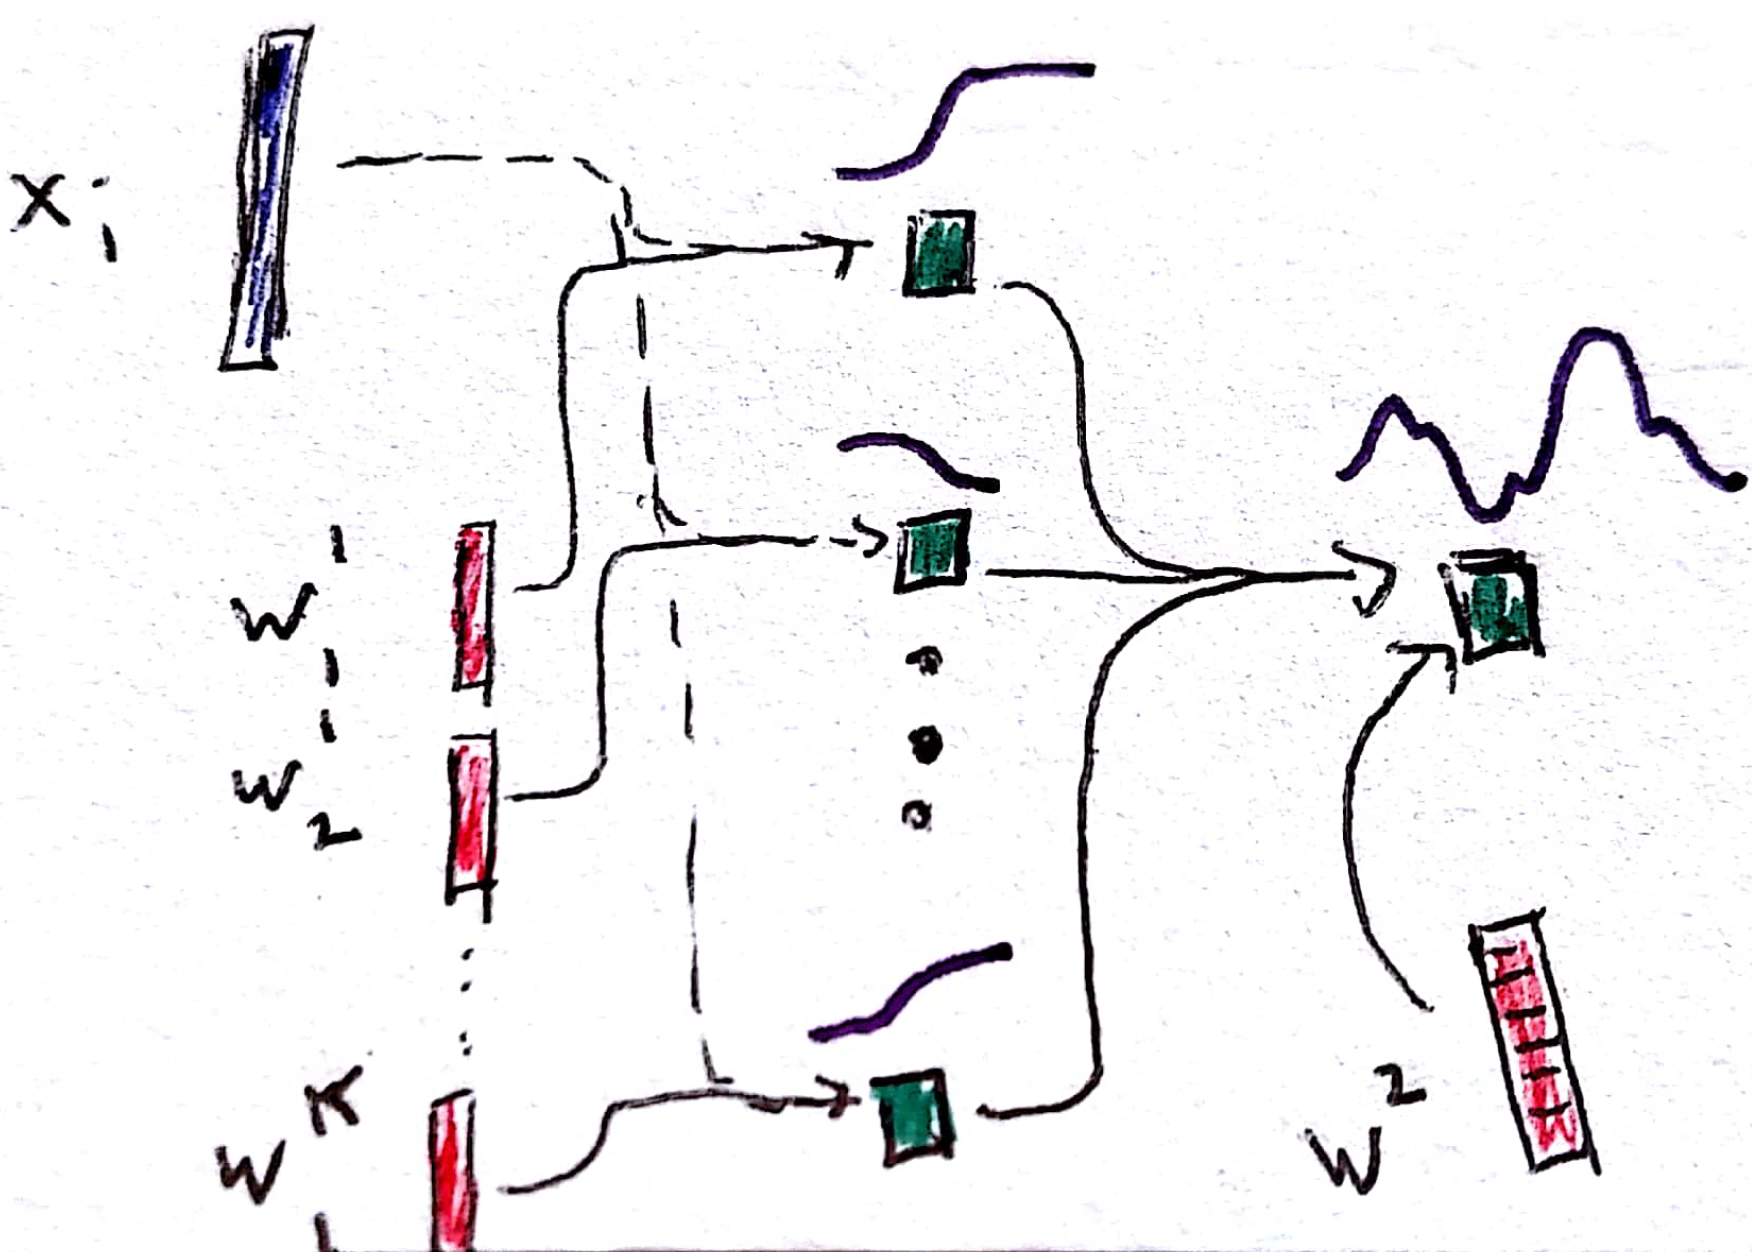
\includegraphics[width=0.55\paperwidth]{figure/mixture_logistic_k}
    \caption{Mixing more sigmoids, we can represent even more complicated
      functions. \label{fig:mixture_logistic_k} }
  \end{figure}
\end{frame}

\begin{frame}
  \frametitle{Nomenclature}
  \begin{itemize}
  \item Reason for the name: Every output layer coordinate can see every input
    layer coordinate
  \item Biologically motivated shorthand: ``layer coordinate'' $\rightarrow$ neuron
  \item The two layers are \textit{fully connected}
  \end{itemize}
\begin{figure}
  \centering
  \includegraphics[width=0.3\paperwidth]{figure/fully_connected1}
  \caption{Our earlier notation for a fully connected layer.}
  %%   one. \label{fig:fully_connected}}
\end{figure}
\end{frame}

\begin{frame}
  \frametitle{Nomenclature}
  \begin{itemize}
  \item Reason for the name: Every output layer coordinate can see every input
    layer coordinate
  \item Biologically motivated shorthand: ``layer coordinate'' $\rightarrow$ neuron
  \item The two layers are \textit{fully connected}
  \end{itemize}
\begin{figure}
  \centering
  \includegraphics[width=0.3\paperwidth]{figure/fully_connected2}
  \caption{Each output unit is connected to all of the previous layer's inputs.}
\end{figure}
\end{frame}

\begin{frame}
  \frametitle{Nomenclature}
  \begin{itemize}
  \item Reason for the name: Every output layer coordinate can see every input
    layer coordinate
  \item Biologically motivated shorthand: ``layer coordinate'' $\rightarrow$ neuron
  \item The two layers are \textit{fully connected}
  \end{itemize}
\begin{figure}
  \centering
  \includegraphics[width=0.3\paperwidth]{figure/fully_connected3}
  \caption{All the outputs from one layer can affect all the inputs to the next
    one. \label{fig:fully_connected3}}
\end{figure}
\end{frame}

\begin{frame}
  \frametitle{Fully Connected Layers: Formula}
  \begin{itemize}
  \item This has concise mathematical notation
    \begin{align*}
      \sigma\left(W_{k}h_{k - 1}\right)
    \end{align*}
  \item The nonlinearity $\sigma$ is applied elementwise
  \item It's common to explicitly include a bias term $b_{k}$ inside the
    nonlinearity: $\sigma\left(W_k h_{k - 1} + b_k\right)$
  \end{itemize}
\end{frame}

\section{Convolution in 1D}

\begin{frame}
  \frametitle{The Probability of Sums}
  \begin{itemize}
  \item First a digression on 1D sequences
  \item Material largely taken from Chris Olah's (incredible!) blog
    (\url{http://colah.github.io/})
  \end{itemize}
\end{frame}

\begin{frame}
  \frametitle{The Probability of Sums}
  \begin{itemize}
  \item Drop a ball and see where it lands
    \begin{itemize}
    \item Drop it slightly to the right (for reasons that will be clear later)
    \end{itemize}
  \item For simplicity, suppose it lands on some grid
  \item Consider the probabilities of different outcomes
  \end{itemize}
\begin{figure}[ht]
  \centering
  \includegraphics[width=0.6\paperwidth]{figure/drop_once}
  \caption{Branch widths correspond to the probabilities of landing in different
    positions. \label{fig:drop_once} }
\end{figure}
\end{frame}

\begin{frame}
  \frametitle{The Probability of Sums}
  \begin{itemize}
    \item Drop it again, starting from the place it fell last time
    \item Each branch gives a path from original to final position
    \item Branch probability $\rightarrow$ product of original probabilities
    \item E.g., go right by 2 steps then left by 1 is $f\left(2\right)f\left(-1\right)$
  \end{itemize}
  \begin{figure}[ht]
    \centering
    \includegraphics[width=0.6\paperwidth]{figure/drop_twice}
    \caption{Can compute probabilities of landing in different positions, after
      two drops.
       \label{fig:drop_twice_probs}}
  \end{figure}
\end{frame}

\begin{frame}
  \frametitle{The Probability of Sums}
  \begin{itemize}
    \item Probability of landing at a prespecified position after
      two drops?
    \item Consider any of the intermediate positions it could have
      landed at
    \item Sum over all the paths that lead to the same destination
  \end{itemize}
  \begin{figure}[ht]
    \centering
    \includegraphics[width=0.6\paperwidth]{figure/convolution_branches1}
    \caption{Each branch starts at the initial dropping position and ends at
      $u$. \label{fig:convolution_branches} }
  \end{figure}
\end{frame}

\begin{frame}
  \frametitle{The Probability of Sums}
  \begin{itemize}
    \item Probability of landing at a prespecified position after
      two drops?
    \item Consider any of the intermediate positions it could have
      landed at
    \item Sum over all the paths that lead to the same destination
  \end{itemize}
  \begin{figure}[ht]
    \centering
    \includegraphics[width=0.35\paperwidth]{figure/convolution_branches2}
    \caption{Each branch starts at the initial dropping position and ends at
      $u$. \label{fig:convolution_branches} }
  \end{figure}
\end{frame}

\begin{frame}
  \frametitle{Mathematical Formula}
  \begin{itemize}
    \item This can be expressed concisely
      \begin{align*}
        \Parg{X + Y = u} &= \sum_{k = -\infty}^{\infty} f\left(k\right)f\left(u - k\right) \\
        &\stackrel{\text{defined}}{=} f * f \left(u\right)
      \end{align*}
    \item Notice that the upside-down tree is reflected and translated
      \begin{itemize}
      \item Exactly the transformation $f\left(x\right) \rightarrow f\left(u - x\right)$
      \end{itemize}
  \end{itemize}
  \begin{figure}[ht]
    \centering
    \includegraphics[width=0.35\paperwidth]{figure/convolution_branches2_annotated}
    \caption{Each branch starts at the initial dropping position and ends at
      $u$. \label{fig:convolution_branches} }
  \end{figure}
\end{frame}

\begin{frame}
  \frametitle{Varying functions}
  \begin{itemize}
    \item We didn't need to drop in the same way the second time
      \begin{align*}
        \Parg{X + Y = u} &= \sum_{k = -\infty}^{\infty} f\left(k\right)g\left(u - k\right) \\
        &\stackrel{\text{defined}}{=} f * g\left(u\right)
      \end{align*}
  \end{itemize}
  \begin{figure}[ht]
    \centering
    \includegraphics[width=0.5\paperwidth]{figure/convolution_vary_funs}
    \caption{Suppose we first dropped from very high, and then afterwards from
      very low, so that it can't move very far from its second position.
       \label{fig:convolution_vary_funs} }
  \end{figure}
\end{frame}

\section{Convolution in Computer Vision}

\begin{frame}
  \frametitle{Convolution and Computer Vision}
  \begin{itemize}
  \item Convolutions have been very successful in computer vision
  \item Many reasons,
    \begin{itemize}
    \item Weight sharing / local connectivity means far fewer parameters
    \item Can be computed very fast, especially on GPUs
    \item Related to biological vision
    \end{itemize}
  \end{itemize}
\begin{figure}[ht]
  \centering
  \includegraphics[width=0.5\paperwidth]{figure/computer_vision_typical}
  \caption{A typical computer vision architecture. Note the convolution
    layers. \label{fig:label} }
\end{figure}
\end{frame}

\begin{frame}
  \frametitle{Image Convolution}
  \begin{itemize}
  \item Our previous discussion applies for dropping a ball onto a 2D surface
  \item Think of an image as a function over a grid
  \item The function for the second drop designed to have small support
    \begin{itemize}
    \item Typically called ``filters''
    \item These will be learned from data
    \end{itemize}
  \end{itemize}
  \begin{figure}[ht]
    \centering
    \includegraphics[width=0.32\paperwidth]{figure/convolution_image_function}
    \caption{Think of an image as a function in 2D. Each pixel would be the
      endpoint for a branch in the ``dropping ball'' example we've been working
      with. \label{fig:convolution_image_fun} }
  \end{figure}
\end{frame}

\begin{frame}
  \frametitle{Example Computation}
  Check interactive example: \url{http://setosa.io/ev/image-kernels/}
  \begin{figure}[ht]
    \centering
    \includegraphics[width=0.6\paperwidth]{figure/convolution_example}
    \caption{An example convolution with a single (sharpening) filter.
      \label{fig:convolution_examples} }
  \end{figure}
\end{frame}

\begin{frame}
  \frametitle{Blurring}
  \begin{itemize}
    \item You can learn many types of image processing operations using
      prespecified filters
    \item Neural networks \textit{learn} filters that are ideal for given
      classification tasks
  \end{itemize}
  \begin{figure}[ht]
    \centering
    \includegraphics[width=0.4\paperwidth]{figure/blurring_example}
    \caption{Blurring can be implemented by convolving with a small
      plateau. \label{fig:blurring_example} }
  \end{figure}
\end{frame}

\begin{frame}
  \frametitle{Edge Detection}
  \begin{itemize}
    \item You can learn many types of image processing operations using
      prespecified filters
    \item Neural networks \textit{learn} filters that are ideal for given
      classification tasks
  \end{itemize}
  \begin{figure}[ht]
    \centering
    \includegraphics[width=0.4\paperwidth]{figure/edge_detection_example}
    \caption{Edges can be found by convolving with a small
      zigzag. \label{fig:edges_example} }
  \end{figure}
\end{frame}

\begin{frame}
  \frametitle{Local Connectivity}
  \begin{itemize}
  \item Convolutions have small support
  \item Connections between layers are sparse
  \item More biologically plausible than having all neurons connected with one
    another
  \end{itemize}
  \begin{figure}[ht]
    \centering
    \includegraphics[width=0.6\paperwidth]{figure/conv_connectivity}
    \caption{After stacking the image into a long vector, A convolution layer
      creates a local connectivity pattern between layers (contrast with fully
      connected layers). \label{fig:conv_connectivity} }
  \end{figure}
\end{frame}

\begin{frame}
  \frametitle{Max Pooling}
  \begin{itemize}
  \item Doing some sort of downsampling can help in various applications
  \item Most common: Take only largest value from a small patch
    \begin{itemize}
    \item Other options are possible, e.g., averaging
    \end{itemize}
  \end{itemize}
  \begin{figure}
    \centering
    \includegraphics[width=0.3\paperwidth]{figure/max_pooling}
    \caption{Max pooling reduces the size of a feature map by taking only the
      largest value within patch.
      \label{fig:max_pooling}}
  \end{figure}
\end{frame}

\begin{frame}
  \frametitle{Some variants}
  \begin{itemize}
  \item Different types of convolution are useful in different subfields of deep
    learning
    \begin{itemize}
    \item Causal convolution \citep{van2016wavenet}
    \item Dynamic Convolutions \citep{kalchbrenner2014convolutional}
    \item Atrous convolution \citep{chen2018deeplab}
    \item Deconvolution \citep{ronneberger2015u}
    \end{itemize}
  \item Not just computer vision!
  \end{itemize}
  \begin{figure}[ht]
    \centering
    \includegraphics[width=0.9\paperwidth]{figure/conv_collage}
    \caption{Examples of the four types of convolutions above. \label{fig:conv_collage} }
  \end{figure}
\end{frame}

\section{Residual Blocks}
\label{sec:residual_layers}

\begin{frame}
  \frametitle{Residual Blocks}
  \begin{itemize}
  \item Deeper layers learn more meaningful representations
  \item Empirically, can be much harder to train
  \item What to do?
  \end{itemize}
\end{frame}

\begin{frame}
  \frametitle{Learning Residuals}
  \begin{itemize}
  \item Introduce complexity on top of existing approximation
  \item Try to transform the previous layer in an intelligent way
  \item Has a feel of forwards stagewise fitting or boosting, and is inspiration
    for neural ODEs \citep{chen2018neural}
  \end{itemize}
\begin{figure}[ht]
  \centering
  \includegraphics[width=0.5\paperwidth]{figure/truth_approx.png}
  \caption{An example of the difference between the true and the
    observed \label{fig:truth_approx} }
\end{figure}
\end{frame}

\begin{frame}
  \frametitle{Learning Residuals}
  \begin{itemize}
  \item Introduce complexity on top of existing approximation
  \item Try to transform the previous layer in an intelligent way
  \item Has a feel of forwards stagewise fitting or boosting, and is inspiration
    for deep ODEs
  \end{itemize}
\begin{figure}[ht]
  \centering
  \includegraphics[width=0.5\paperwidth]{figure/truth_approx_residual.png}
  \caption{An example of the difference between the true and the
    observed \label{fig:truth_approx} }
\end{figure}
\end{frame}

\begin{frame}
  \frametitle{Learning Residuals}
  \begin{itemize}
  \item Introduce complexity on top of existing approximation
  \item Try to transform the previous layer in an intelligent way
  \item Has a feel of forwards stagewise fitting or boosting, and is inspiration
    for deep ODEs
  \end{itemize}
\begin{figure}[ht]
  \centering
  \includegraphics[width=0.6\paperwidth]{figure/truth_approx_residual_panel.png}
  \caption{We will attempt to directly learn the residual (in red), rather than
    trying to arbitrarily modify the current approximation.
    \label{fig:truth_approx} }
\end{figure}
\end{frame}

\begin{frame}
  \frametitle{A First Attempt}
  \begin{itemize}
  \item Introduce a direct connection $h_{k - 1} \rightarrow h_k$
    \begin{align*}
      h_{k} &= f^{k}\left(h_{k - 1}, W_{k}\right) + h_{k - 1}
    \end{align*}
  \item Issues?
  \end{itemize}
\end{frame}

\begin{frame}
  \frametitle{A First Attempt}
  \begin{itemize}
  \item Introduce a direct connection $h_{k - 1} \rightarrow h_k$
    \begin{align*}
      h_{k} &= f^{k}\left(h_{k - 1}, W_{k}\right) + h_{k - 1}
    \end{align*}
  \item Issues?
    \begin{itemize}
    \item Can't adapt different mixing weights on residual
    \item Input and output dimensions might not agree
    \end{itemize}
  \end{itemize}
\end{frame}

\begin{frame}
  \frametitle{Improved Architecture}
  \begin{itemize}
  \item No longer a direct addition, but encourages focusing on residual
    \begin{align*}
      h_{k} &= W^{r}_{k,1}f^{k}\left(h_{k - 1}, W_{k}\right) + W^{r}_{k,2}h_{k - 1}
    \end{align*}
  \item If input and output dimensions match, don't need $W^{r}_{k,2}$
    \begin{figure}[ht]
      \centering
      \includegraphics[width=0.4\paperwidth]{figure/resnet_block}
      \caption{Resnet building block, according to the improved
        architecture.\label{fig:resnet_block} }
    \end{figure}
  \end{itemize}
\end{frame}

\begin{frame}
  \frametitle{Applications}
  \begin{itemize}
  \item Facilitates training for very deep networks
  \item Used successfully in several competitions
  \end{itemize}
  \begin{figure}[ht]
    \centering
    \includegraphics[width=0.18\paperwidth]{figure/resnet_application}
    \caption{The middle column escribes a naive approach to a very deep network,
      which fails to train. The residual network (right) is better than the other
      two. \label{fig:resnet_application} }
  \end{figure}
\end{frame}

\begin{frame}
  \frametitle{Conclusion}
 \begin{itemize}
 \item Modularity in backprop $\rightarrow$ design independent layers
 \item Convolution and residual layers enjoy empirical success in range of
   domains
 \item Many types of layers that we haven't discussed, but all work using the
   same chain rule and local updating types of ideas
   \begin{itemize}
   \item Sequential data: LSTM Cells \citep{schmidhuber1997long}, Gatted
     Recurrent Units \citep{chung2014empirical}
   \item Attention mechanisms \citep{bahdanau2014neural}
   \item Feature-wise Modulation \citep{perez2017film}
   \end{itemize}
 \end{itemize}
\end{frame}

\begin{frame}
\bibliographystyle{plain}
\bibliography{refs}
\end{frame}

\end{document}
